% - - - - - - - - - - - - - - - - - - - - - - - - - - - - - - - - - - - - - - - 
% Core setup
% - - - - - - - - - - - - - - - - - - - - - - - - - - - - - - - - - - - - - - - 
\documentclass[norsk,11t,a4paper]{article}
\usepackage[tmargin=2.5cm,rmargin=2.5cm,bmargin=2.5cm,lmargin=2.5cm]{geometry}
\usepackage[norsk]{babel}         % Support for other languages than english
\usepackage[utf8]{inputenc}       % Input encoding
\usepackage[T1]{fontenc}          % Font encoding
\usepackage{microtype}            % Improve text appearance in numerous ways
\usepackage{textcomp}             % Add extra symbols
\usepackage{mathtools}            % Improvements for math
\usepackage{amssymb}              % Extended math symbols


% - - - - - - - - - - - - - - - - - - - - - - - - - - - - - - - - - - - - - - - 
% Font packages
% - - - - - - - - - - - - - - - - - - - - - - - - - - - - - - - - - - - - - - - 
\usepackage[osf]{newpxtext}       % Main (serif/sans-serif) font
\usepackage{newpxmath}            % Math font
\usepackage[scaled]{beramono}     % Monospace font


% - - - - - - - - - - - - - - - - - - - - - - - - - - - - - - - - - - - - - - - 
% Additional packages
% - - - - - - - - - - - - - - - - - - - - - - - - - - - - - - - - - - - - - - - 
\usepackage[T1]{url}              % Clickable URLs
\usepackage{hyperref}             % Clickable references
\usepackage{csquotes}             % Support quote marks in various languages
\usepackage{ulem}                 % Double underline
\usepackage[makeroom]{cancel}     % Crossing out text
\usepackage{nicefrac}             % Nice looking fractals
\usepackage{gensymb}              % Degree symbol
\usepackage[compact]{titlesec}    % Title style
\usepackage{setspace}             % Set paragraph spacing
\usepackage{xcolor}               % Colors
\usepackage{enumitem}             % Lists
\usepackage{listings}             % Insert code
\usepackage{tikz}                 % Drawing of graphics
\usepackage{graphicx}             % Insert images
\usepackage{pdfpages}             % Insert pdf pages
\usepackage{biblatex}             % Bibliography


% - - - - - - - - - - - - - - - - - - - - - - - - - - - - - - - - - - - - - - - 
% Apprentice colorscheme (https://github.com/romainl/Apprentice)
% - - - - - - - - - - - - - - - - - - - - - - - - - - - - - - - - - - - - - - - 
\definecolor{color0}{HTML}{1C1C1C}
\definecolor{color1}{HTML}{AF5F5F}
\definecolor{color2}{HTML}{5F875F}
\definecolor{color3}{HTML}{87875F}
\definecolor{color4}{HTML}{5F87AF}
\definecolor{color5}{HTML}{5F5F87}
\definecolor{color6}{HTML}{5F8787}
\definecolor{color7}{HTML}{6C6C6C}
\definecolor{color8}{HTML}{444444}
\definecolor{color9}{HTML}{FF8700}
\definecolor{color10}{HTML}{87AF87}
\definecolor{color11}{HTML}{FFFFAF}
\definecolor{color12}{HTML}{87AFD7}
\definecolor{color13}{HTML}{8787AF}
\definecolor{color14}{HTML}{5FAFAF}
\definecolor{color15}{HTML}{FFFFFF}
\definecolor{colorfg}{HTML}{BCBCBC}
\definecolor{colorbg}{HTML}{262626}


% - - - - - - - - - - - - - - - - - - - - - - - - - - - - - - - - - - - - - - - 
% Habamax colorscheme (https://github.com/habamax/vim-habamax)
% - - - - - - - - - - - - - - - - - - - - - - - - - - - - - - - - - - - - - - - 
\definecolor{bright_cyan}{HTML}{87AFAF}
\definecolor{dark_cyan}{HTML}{5F8787}
\definecolor{cyan}{HTML}{1F3F5F}
\definecolor{pink}{HTML}{D75F87}
\definecolor{red}{HTML}{D75F5F}
\definecolor{dark_red}{HTML}{AF5F5F}
\definecolor{bright_green}{HTML}{5FF75F}
\definecolor{green}{HTML}{87D787}
\definecolor{dark_green}{HTML}{5FAF5F}
\definecolor{blue}{HTML}{5fafd7}
\definecolor{dark_blue}{HTML}{5F87AF}
\definecolor{bright_yellow}{HTML}{ffaf5f}
\definecolor{yellow}{HTML}{d7af87}
\definecolor{dark_yellow}{HTML}{af875f}
\definecolor{bright_magenta}{HTML}{ff00af}
\definecolor{magenta}{HTML}{d787d7}
\definecolor{dark_magenta}{HTML}{af87af}


% - - - - - - - - - - - - - - - - - - - - - - - - - - - - - - - - - - - - - - - 
% Package settings
% - - - - - - - - - - - - - - - - - - - - - - - - - - - - - - - - - - - - - - - 
\usetikzlibrary{er, positioning}
\renewcommand{\arraystretch}{1.25}
\color{color0}
\linespread{1.05}
\setlength{\parindent}{0pt}
\setlength{\tabcolsep}{18pt}
\newlength{\myeqskip}\setlength{\myeqskip}{2pt}
\titlespacing*{\section}{0cm}{1.5cm}{0.25cm}
\titlespacing*{\subsection}{0cm}{1cm}{0.5cm}
\titleformat{\section}{\normalfont\large\bfseries}{\thesection}{0.75em}{}
\titleformat{\subsection}{\normalfont\normalsize\itshape}{\thesubsection.}{0.75em}{}
\titleformat{\subsubsection}{\normalfont\normalsize\itshape}{\thesubsubsection.}{0.75em}{}
\lstset{literate={æ}{{\ae}}1{Æ}{{\AE}}1{ø}{{\o}}1{Ø}{{\O}}1{å}{{\aa}}1{Å}{{\AA}}1,
keywordstyle={\bfseries\color{dark_red}}, 
commentstyle={\bfseries\color{dark_cyan}},
basicstyle={\scriptsize\ttfamily\color{color0}}, 
numbers=none,numberstyle={\scriptsize\ttfamily\color{color7}},
aboveskip=0.1cm,belowskip=1.0cm,columns=fixed,
breaklines=true,breakatwhitespace=false,keepspaces=true,
showspaces=false,showstringspaces=false,tabsize=4,
captionpos=b,inputencoding=utf8,extendedchars=true}


% - - - - - - - - - - - - - - - - - - - - - - - - - - - - - - - - - - - - - - - 
% Custom commands
% - - - - - - - - - - - - - - - - - - - - - - - - - - - - - - - - - - - - - - - 
\newcommand{\oppgave}[1]{\subsection*{Oppgave #1}}
\newcommand{\oppgaveDelStart}{\begin{enumerate}[leftmargin=*,itemsep=1.5cm,labelsep=1.5em,label=\alph*)]}
\newcommand{\oppgaveDelSlutt}{\end{enumerate}}
\newcommand{\oppgaveDel}[1]{\item[#1)]}


% - - - - - - - - - - - - - - - - - - - - - - - - - - - - - - - - - - - - - - - 
% Set title / author
% - - - - - - - - - - - - - - - - - - - - - - - - - - - - - - - - - - - - - - - 
\title{DAT107 - Obligatorisk innlevering 2}
\author{\normalsize Gruppemedlemmer: \\ Stephen Neba Fuh, Tord Johan Melheim, \\ Ebubekir Siddik Yuksel, Casper Eide Özdemir-Børretzen}
\date{}


% - - - - - - - - - - - - - - - - - - - - - - - - - - - - - - - - - - - - - - - 
% Document start and title page
% - - - - - - - - - - - - - - - - - - - - - - - - - - - - - - - - - - - - - - - 
\begin{document}
\maketitle


% - - - - - - - - - - - - - - - - - - - - - - - - - - - - - - - - - - - - - - - 
% Main content
% - - - - - - - - - - - - - - - - - - - - - - - - - - - - - - - - - - - - - - - 

%\begin{lstlisting}[language=SQL]
%\end{lstlisting}
%\lstinputlisting[language=SQL]{file.sql}
%\oppgave{1}
%\oppgaveDelStart
%\oppgaveDel{a}
%\oppgaveDel{b}
%\oppgaveDel{c}
%\oppgaveDelSlutt

% Huskeliste:
% Primærnøkler
% Fremmednøkler
% Datatyper
% Min/maks kadinalitet
% Sterke/svake entitetstyper og eksistensavhengighet/uavhengighet (kråkefot-notasjon) eller type aggregering (UML-notasjon)
% Redegjørelse/forklaring på at ER-modellen tilfredsstiller hver av 1., 2., og 3. normalform. Tabellene skal faktisk være korrekt normaliserte – det holder ikke å hevde at de er normaliserte dersom de ikke er det.
% Redegjørelse for de valgene som er tatt. Det blir lagt vekt på både praktisk utførelse og teoretisk forståelse
% Besvarelsen skal være “konsistent”, dvs. skal være for den “samme” databasen, og de valgene man har tatt i en del av besvarelsen skal ikke “motsies” av de valgene man har tatt i en annen del av besvarelsen.

\section{Introduksjon}

Problemstilling: En forening har behov for et system for å administrere medlemmer. Det er tenkt å ta i bruk en SQL database for å bygge dette systemet.
Foreningen har flere lokallag, og alle medlemmer er med i nøyaktiv ett lokallag.
Lokallag har navn, leder (medlem), samt postnummer/sted og gatenavn/husnummer for møtelokale.
Et medlem har medlemsnummer, fornavn, etternavn, telefonnummer, e-postadresse, postnummer/sted, gatenavn/husnummer, og medlemsstatus (aktiv/utmeldt).
For hvert medlem skal det i tillegg loggføres om medlemsavgift hare blitt betalt for hvert år.\\

Oppgaver: Oppgaven vi skal ta for oss er å tegne en logisk (fullstendig) ER-modell i ???-notasjon for en SQL database som fyller kravene spesifisert i problemstillingen, samt å vise at modellen tilfredsstiller 3. normalform.

\section{Metode}

TODO: Beskriv metodene som skal brukes for å løse oppgavene

\vspace{0.5cm}
\begin{tabular}{|c|c|c|} 
\hline
&Fordel&Ulempe \\
\hline
    a&b&c\\
    a&b&c\\
    a&b&c\\
\hline
\end{tabular}

\section{Resultat}

TODO: Beskriv resultatet på deloppgavene etter å ha benyttet metodene

\tikzstyle{every entity} = [color9]
\tikzstyle{every attribute} = [color12]
\tikzstyle{every relationship} = [color14]

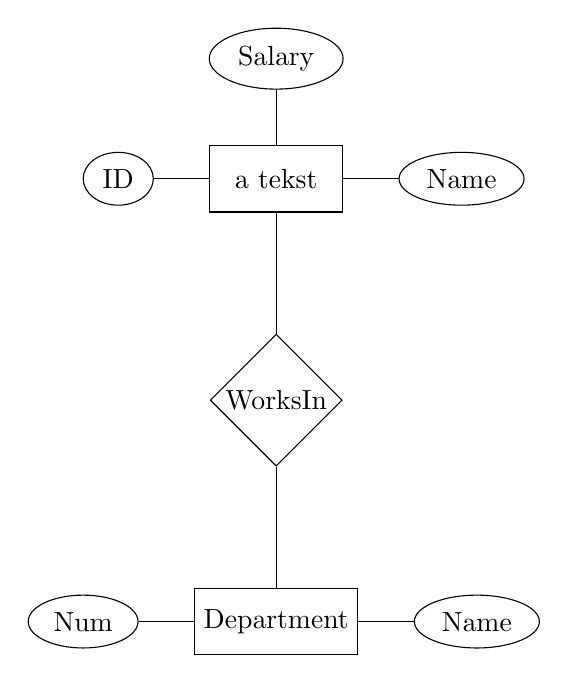
\begin{tikzpicture}[node distance=6em]
  \node[entity] (emp) {a tekst};
  \node[attribute] (e_id) [left=2em of emp] {\key{ID}} edge (emp);
    \node[attribute] (e_name) [right=2em of emp] {Name} edge (emp);
    \node[attribute] (e_sal) [above=2em of emp] {Salary} edge (emp);
  \node[relationship] (works) [below of=emp, node distance=8em] {WorksIn} edge (emp);
  \node[entity] (dept) [below of=works, node distance=8em] {Department} edge (works);
    \node[attribute] (d_num) [left=2em of dept] {\key{Num}} edge (dept);
    \node[attribute] (d_name) [right=2em of dept] {Name} edge (dept);

\end{tikzpicture}

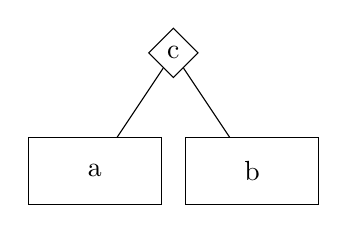
\begin{tikzpicture}
  \node[entity] (sheep)  at (0,0)   {a};
  \node[entity] (genome) at (2,0)   {b};
  \node[relationship]    at (1,1.5) {c}
    edge (sheep)
    edge (genome);
\end{tikzpicture}

\begin{lstlisting}[language=SQL]
    -- SQL eksempelkode
    SELECT * FROM ...;
\end{lstlisting}

\section{Diskusjon}
TODO: Oppsummer resultatene, funnene og vurderingene


% - - - - - - - - - - - - - - - - - - - - - - - - - - - - - - - - - - - - - - - 

\end{document}
